\newpage
\lecture{4}{Произведения сигма-алгебр.}

\begin{definition}
    \label{lect4:def:mult}
    Пусть $X,\,Y,\,Z$~--- множества, $\CE\subset \CP(X),\, \F\subset\CP(Y),\, \CG\subset \CP(Z)$.
    \begin{align*}
        P_{\CE,\,\F}        & := \{A\times B\ \vert\ A\in\CE,\,B\in\F \}                   \\
        P_{\CE,\,\F,\, \CG} & := \{A\times B\times C\ \vert\ A\in\CE,\,B\in\F,\,C\in\CG \}
    \end{align*}
\end{definition}

\begin{definition}
    Если $\CE,\,\F$ и $\CG$~--- $\sigma$"=алгебры, то
    \begin{align*}
        \CE\otimes\F           & :=\sigma(P_{\CE,\,\F})        \\
        \CE\otimes\F\otimes\CG & :=\sigma(P_{\CE,\,\F,\,\CG}),
    \end{align*}
    называется \mdef{произведением сигма-алгебр} $\CE$ и $\F$, и $\CE,\, \F$ и $\CG$ соответственно.
\end{definition}

Докажем некоторые свойства произведения сигма-алгебр.

\begin{claim}
    Если $\CE,\,\F,\,\CG$~--- $\sigma$"=алгебры, то
    \[
        (\CE\otimes\F)\otimes\CG=\CE\otimes(\F\otimes\CG)=\CE\otimes\F\otimes\CG.
    \]

    \begin{proof}
        Докажем, что $(\CE\otimes\F)\otimes\CG=\CE\otimes\F\otimes\CG$.
        По определению:
        \begin{align}
            (\CE\otimes\F)\otimes\CG & =\sigma(\{A\times B\ \vert\ A\in\CE\otimes\F,\, B\in\CG\}),\label{lect4:efg} \\
            \CE\otimes\F             & =\sigma(\{M\times N\ \vert\ M\in\CE,\, N\in\F\}).
        \end{align}
        Откуда следует, что $\forall M\in\CE,\, N\in\F$ выполнено $M\times N\in\CE\otimes\F$.
        Теперь подставим вместо $A$ в формуле \eqref{lect4:efg} $M\times N$. Получим
        $\forall B\in\CG:\ M\times N\times B\in(\CE\otimes\F)\otimes \CG$. То есть доказано вложение
        $P_{\CE,\,\F,\,\CG}\subset (\CE\otimes\F)\otimes \CG$, а это и означает, что
        $\CE\otimes\F\otimes\CG\subset (\CE\otimes\F)\otimes \CG$, так как слева и справа сигма-алгебры,
        содержащие $P_{\CE,\,\F,\,\CG}$, но слева по определению минимальная по вложению сигма-алгебра.

        Осталось доказать вложение в обратную сторону. Сначала докажем, что
        \[
            \{A\times B\ \vert\ A\in\CE\otimes\F,\, B\in\CG\}\subset\CE\otimes\F\otimes\CG.
        \]
        Из этого сразу будет следовать и вложение сигма-алгебр (снова в силу минимальности по вложению).
        Обозначим $\CM=\CE\otimes\F\otimes\CG$.
        Зафиксируем $B\in\CG$. Нужно доказать, что $A\times B\in\CM$ для $\forall A\in\CE\otimes\F$.
        Рассмотрим множество $Q$, состоящее из всех $A$, обладающих таким свойством, то есть
        \[
            Q=\{A\in\CE\otimes\F\ \vert\ A\times B\in\CM\}.
        \]
        Заметим, что $Q$ является $\sigma$"=алгеброй:
        \begin{enumerate}[label=\arabic*\degree.]
            \item $\varnothing\in Q$.
            \item Так как $A\subset X\times Y$ (смотри определение \ref{lect4:def:mult}),
                  $A\in Q\Rightarrow A^C\times B=(X\times Y\times B)\setminus (A\times B)\in\CM\Rightarrow A^C\in Q$.
            \item Аналогично для объединения: $\{A_n\}_{n\in\N},\, A_n\in Q$:
                  \[
                      \left(\bigcup_{n=1}^{\infty}A_n\right)\times B=\bigcup_{n=1}^{\infty}\left(A_n\times B\right)\in\CM
                      \Rightarrow\bigcup_{n=1}^{\infty}A_n\in Q.
                  \]
        \end{enumerate}

        С другой стороны, $P_{\CE,\, \F}\subset Q$, в самом деле, если $A=E\times F$, где $E\in\CE$, $F\in\F$, то
        $A\times B = E\times F\times B\in \CM$.
        Тогда $\CE\otimes\F\subset Q$, потому что $Q$~--- $\sigma$"=алгебра.

        Аналогично доказывается, что $\CE\otimes(\F\otimes\CG)=\CE\otimes\F\otimes\CG$, откуда и следует вся
        цепочка равенств.

    \end{proof}
\end{claim}

\subsection{Сечения множеств.}

\begin{figure}[!ht]
    \centering
    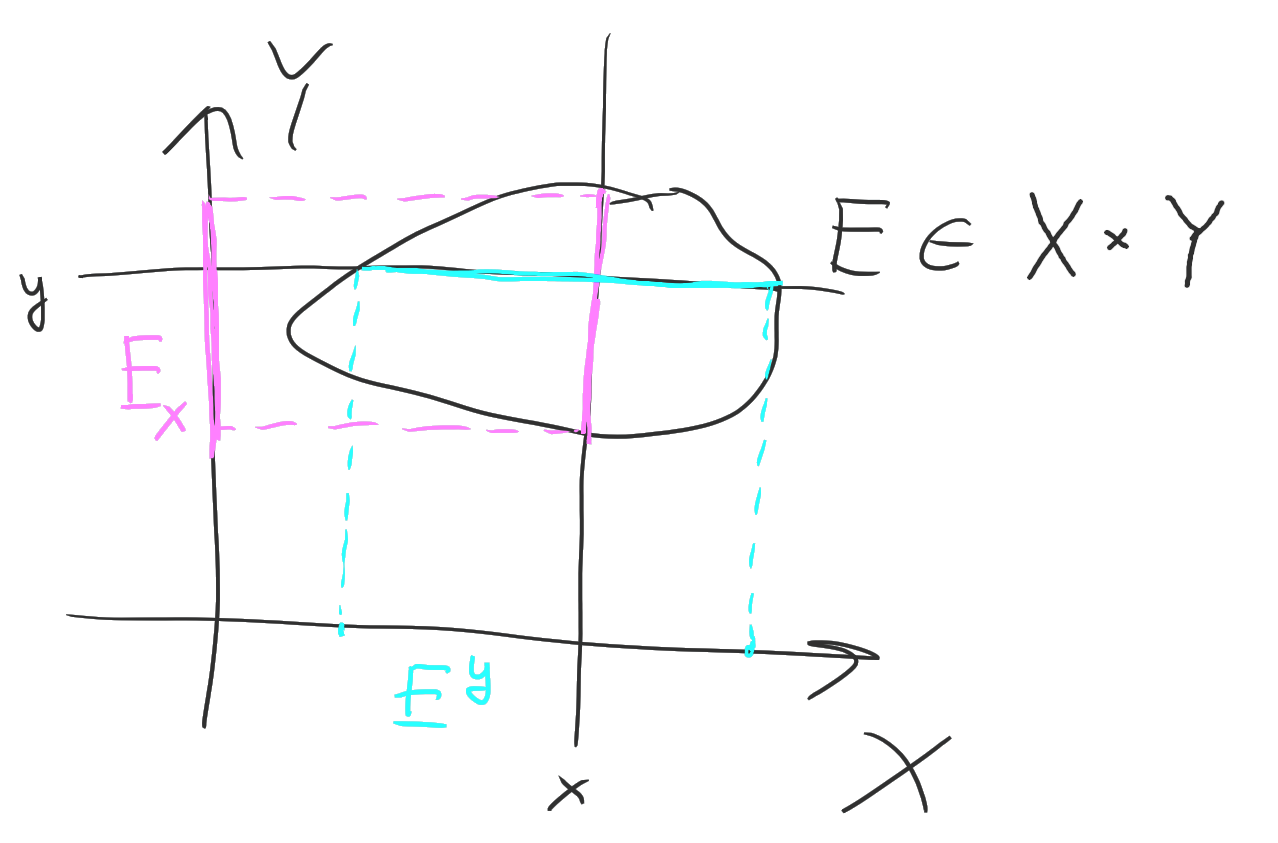
\includegraphics[width=0.7\textwidth]{mult.png}
    \caption{Множество $E$.}
    \label{lect4:fig:mult}
\end{figure}

\begin{definition}
    Пусть $E\in X\times Y,\, x\in X,\, y\in Y$. 
    \begin{align*}
        E_x&:=\{y\in Y:\ (x,\, y)\in E\}\\
        E^y&:=\{x\in X:\ (x,\, y)\in E\}
    \end{align*}
    Для лучшего понимания смотри рисунок \ref{lect4:fig:mult}. Будем такие конструкции называть \mdef{вертикальными 
    и горизонтальными сечениями} соответственно.
\end{definition}

\begin{remark}
    Легко заметить пару свойств введенных понятий:
    \begin{enumerate}[label=\arabic*\degree.]
        \item $(E^C)_x = \{y\in Y:\ (x,\, y)\notin E\}=(E_x)^C.$
        \item Если $\{E_n\}_{n\in\N}:\ E_n\subset X\times Y$, то 
        $\left(\bigcup\limits_{n=1}^{\infty}E_n\right)_x=\bigcup\limits_{n=1}^{\infty}\left(E_n\right)_x$
        \item Если $\{E_n\}_{n\in\N}:\ E_n\subset X\times Y$, то 
        $\left(\bigcap\limits_{n=1}^{\infty}E_n\right)_x=\bigcap\limits_{n=1}^{\infty}\left(E_n\right)_x$
    \end{enumerate}
    И аналогично для горизонтальных сечений.
\end{remark}

Зададимся следующим вопросом. Верно ли, что $E_x\in\F$ и $E^y\in\CG$, если $E\in\CE\otimes\F$?

\begin{theorem}
    Пусть $\CE\in\CP(X)$ и $\F\in\CP(Y)$~--- $\sigma$"=алгебры. Тогда $\forall E\in\CE\otimes\F\ \forall x\in X\ \forall y\in Y$ 
    выполнено $E_x\in\F$ и $E^y\in\CE$.

    \begin{proof}
        Докажем только, $E_x\in\F$ (вторая вложенность будет доказываться аналогично). 
        Пусть $\CH = \{E\in\CE\otimes\F:\ E_x\in\F\}$. Заметим, что $\CH$~--- $\pi$"=система:
        если $E,\, F\in\CH$, то в силу замечания имеем $(E\cap F)_x=E_x\cap F_x\in\F$. 
        
        Докажем, что $\CH$~--- еще и $\lambda$"=система (то есть $\sigma$"=алгебра). Легко видеть, что $\varnothing\in\CH$.
        Рассмотрим $\{E_n\in\CH\}_{n\in\N}:\ E_i\cap E_j=\varnothing,\ \forall i\neq j$. Пусть тогда
        $E:=\bigsqcup\limits_{n=1}^{\infty}E_k$. Аналогично, 
        \[
            E_x=\bigsqcup_{n=1}^{\infty}(E_k)_x\in\F\text{, так как } \F\text{~--- $\sigma$"=алгебра ($E_{kx}\in\F$).}
        \]

        Итак, $\CH$~--- $\sigma$"=алгебра, а также $\CH\supset \{P\times Q\ \vert\ P\in\CE,\, Q\in\F\}$, 
        поэтому $\CH$ содержит и сигма-алгебру, порожденную этим множеством:
        $H\supset \sigma(\{P\times Q\ \vert\ P\in\CE,\, Q\in\F\})=\CE\otimes\F$.

    \end{proof}
\end{theorem}

\subsection{Монотонные классы.}

\begin{definition}
    Семейство $\F$ подмножества множества $X$ называется \mdef{монотонным классом}, если 
    $\forall \{E_k\}_{k\in\Z}\subset\F$ такой, что $E_k\subset E_{k+1}\ \forall k\in\Z$,
    выполнено $\bigcup\limits_{k\in\Z}E_k\in\F$ и $\bigcap\limits_{k\in\Z}E_k\in\F$.

    Простыми словами, множество замкнуто относительно объединения и пересечения последовательностей 
    вложенных множеств.
\end{definition}

\begin{theorem}[о монотонном классе]
    Пусть $\F\subset\CP(X)$~--- алгебра, $\CM\subset\CP(X)$~--- монотонный класс и $\F\subset \CM$.
    Тогда $\sigma(\F)\subset\CM$.

    \begin{remark}
        Доказательство аналогично доказательству теоремы Дынкина.
    \end{remark}
\end{theorem}

\subsection{Мера.}

\begin{definition}
    Пусть $X$~--- множество и $\F\subset\CP(X)$. Функция $\mu:\ \F\rightarrow[0,\,+\infty]$
    называется
    \begin{enumerate}
        \item \mdef{монотонной} (на $\F$), если для любых $A,\, B\in\F$ таких, что 
        $A\subset B$, выполнено $\mu(A)\leqslant \mu(B)$;

        \item \mdef{конечно-субаддитивной} (на $\F$), если для любого конечного
        семейства $\{A_k\}_{k=1}^n\subset\F$ такого, что $\bigcup\limits_{k=1}^n A_k\in\F$, 
        выполнено
        \[
            \mu\left(\bigcup_{k=1}^nA_k\right)\leqslant\sum_{k=1}^n\mu(A_k);
        \]
        
        \item \mdef{конечно-аддитивной} (на $\F$), если для любого \textbf{дизъюнктного} 
        конечного семейства $\{A_k\}_{k=1}^n\subset\F$, такого что 
        $\bigsqcup\limits_{k=1}^n A_k\in\F$ выполнено 
        \[
            \mu\left(\bigsqcup_{k=1}^nA_k\right)=\sum_{k=1}^n\mu(A_k);
        \]
        
        \item \mdef{счётно-субаддитивной} (на $F$), если для любого счётного семейства
        $\{A_k\}_{k\in\N}\subset\F$ такого, что $\bigcup\limits_{k=1}^{\infty} A_k\in\F$,
        выполнено 
        \[
            \mu\left(\bigcup_{k=1}^{\infty}A_k\right)\leqslant\sum_{k=1}^{\infty}\mu(A_k);
        \]
        
        \item \mdef{счётно-аддитивной} (на $F$), если для любого \textbf{дизъюнктного} счётного
        семейства $\{A_k\}_{k\in\N}\subset\F$ выполнено
        \[
            \mu\left(\bigsqcup_{k=1}^{\infty}A_k\right)=\sum_{k=1}^{\infty}\mu(A_k);
        \]
        
        \item \mdef{конечной}, если $X\in\F$ и $\mu(X)<+\infty$;
        \item \mdef{сигма-конечной}, если существует последовательность $\{X_n\}_{n\in\N}\subset\F$
        такая, что $\mu(X_n)<+\infty$ при любом $n\in\N$ и $X=\bigcup\limits_{n=1}^{\infty}X_n$.
    \end{enumerate}
\end{definition}